This section assess the initial simulation implementation, with a single user, a
data rate of approximately 1.6Kbps, and a distance of 50 meters between the user
and the access point. The bitrate is then modified to assess its affect on the
system.

\subsubsection{Part 1:}

Within the wifi-example-sim.cc file, the simulation is given a run time of 20
seconds, a packet size of 1000 bytes and a 0.05 second delay between the
transmission of packets. This corresponds to a total of 400 packets sent over
the space of 20 seconds.

\begin{gather*}
	R=\frac{rxPackets*packetSize*8}{delay} \\
	\frac{400*1000*8}{4.9\times10^{-4}} \\
	6.53\times10^{9}bits
\end{gather*}
\captionof{equation}{Bitrate of Data Traffic (Kbps)}

\begin{gather*}
	Throughput=\frac{rxPackets*packetSize*8}{txTime} \\
	\frac{400*1000*8}{20} \\
	\frac{3,200,000}{20} \\
	160,000 \\
	160Kbps
\end{gather*}
\captionof{equation}{Average Throughput (Kbps)}

The throughput value from the equation above can be seen plot against the users
distance from the access point in Figure \ref{fig:QAthroughput} (plot in Mbps).
\begin{figure}[H]
	\centering
	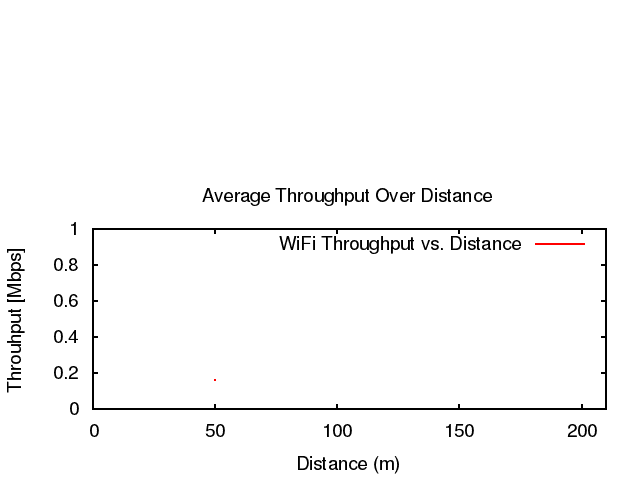
\includegraphics[width=0.8\textwidth]{images/EE500/QA/P1/Images/wifi-throughput}
	\caption{Throughput for a single user at a distance of 50 meters}
	\label{fig:QAthroughput}
\end{figure}

\par Delay time is given within the wifi-example-sim.cc file as measured in
nanoseconds. Form the output, this value is 490381ns. This can be calculated as
follows:
\begin{gather*}
	\overline{delay}=\frac{delaySum}{rxPackets} \\
	\frac{196,152,732}{400} \\
	= \quad 490,381.83ns \\
	= \quad 4.9\times10^{-4}s
\end{gather*}
\captionof{equation}{Average Delay (s)}

\begin{figure}[H]
	\centering
	\includegraphics[width=0.8\textwidth]{images/EE500/QA/P1/Images/wifi-Delay}
	\caption{Delay for a single user at a distance of 50 meters}
	\label{fig:QAdelay}
\end{figure}


Packet loss ratio is given by the following formula:
\begin{gather*}
	PLR = \frac{lostPackets}{rxPackets+lostPackets0} \\
	\frac{0}{400+0} \\
	= \quad 0
\end{gather*}
\captionof{equation}{Average Packet Loss Ratio}

As seen in both the equation above, and in Figure \ref{fig:QALoss}, there is no
packet loss within this simulation.

\begin{figure}[H]
	\centering
	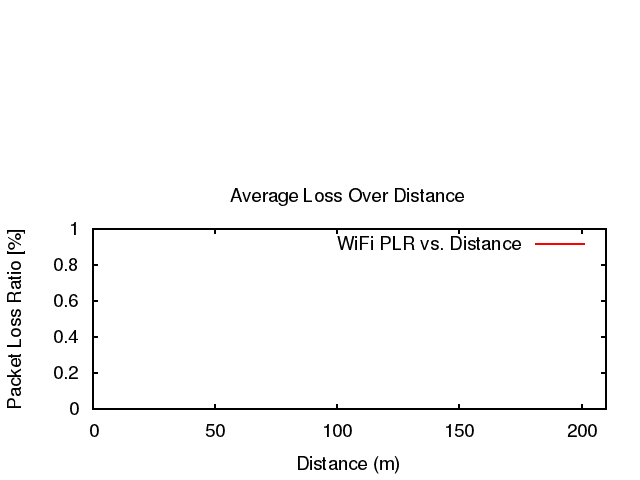
\includegraphics[width=0.8\textwidth]{images/EE500/QA/P1/Images/wifi-loss}
	\caption{Packet Loss Ratio for a single user at a distance of 50 meters}
	\label{fig:QALoss}
\end{figure}
